\setstretch{2}
\section{Outline / Bullet Points}

\subsection{Experimental Protocol}
\begin{itemize}
    \item Albino Rats were anaesthetised using isoflourane and their oxygenation was controlled using a nosecone that supplies oxygen at variable concentration.
    \item Rat is stabilised and a contact lens - contributing no refractive power - and a Viscotears - was used to prevent the eye's becoming dry and irritated. 
    \item Tropicamide was used to dilate the pupil from its usual X diameter to Y diameter
    \item A 2'' diameter 85mm field lens was fitted in front of the fundus camera to allow the smaller pupil and eye ball size to be accommodated in the SFLIO imaging system. 
    \item This lens does induce some glare due to additional reflections of the lens surface in the brightfield image which could ordinarily be corrected by imaging a blacked out room with the illumination on - reproducing the glare - and linearly subtracting it from each image using i.e I - aG where a is found by minimising the standard deviation of the image.
    \item for the purpose of registration this glare polluted area can simply be masked out during the phase cross-correlation process.
    \item Registration images were recorded in brightfield with frame rate of 10hz and a frame integration time of 50ms. This integration time in normal human imaging would be degraded by blur due to saccades but since the rats are anaesthetised this systemic is overridden and the only observed motion artefacts are from what appears to be laboured breathing 
    \item For SFLIM the static affine transformation between the two camera was re-determined using the same convallaria slide mounted in a phantom eye - without using the field lens - this was to account for any small changes in the positions of the SPAD and sCMOS wrt to the imaging path due to having transported the equipment to London from Glasgow. 
    \item SFLIM images were recorded over periods of 150seconds where the laser shutter is initially closed and opened after the a brief period illuminating the retina. This enables at least 2mins of continuous integration using the FLIMera raw mode
\end{itemize}
\subsection{Results}

\begin{itemize}
    \item While a high quality image could be formed on the sCMOs camera which clearly shows the vascular structure of the retina could be formed - albeit polluted by glare in the centre of the vision. A sufficient image could not be formed on the FLIMera but there is sufficient signal to attempt SFLIM unmixing. This could be due to the low fluorescence contrast as evidenced by the fluorescence intensity image recorded with a lp500 filter in the SCMOs camera. 
    \item Can't map FAD across the retina but can use the signal to extract a general trend in the FAD concentration wrt oxygenation.
    \item In the histograms recorded by the FLIMera there was also the addition Gaussian like thermal noise characteristic that was ultimately corrected by simply neglecting these values in the calculation of the cost function of the minimisation process (phi). While this does decrease the overall energy in the signal what is left should be capable of capturing both the long and short lifetime dynamics.
    \item A brief comparison of the possible dark field correction methods yielded no significant change in the recovered concentration of retinal FAD  - dark-field correction by fitting a modified Gaussian to the artefact and subtracting from each histogram, masking the effected time bins, and simple fitting through the artefact.
\end{itemize}


\section{FAD as a marker of retinal health}
Mapping the concentration of FAD would enable diagnosis at the initial stages of retinal disease where metabolic function is compromised before patient's present with permanent physical damage to vision. The mechanism for this lies with FAD being a byproduct of the creation of the bodied energy source, ATP~\cite{berg2007biochemistry}, through aerobic respiration (\cref{eq:resp}. In the early stages of retinal disease the disruption of metabolic processes would disrupt ATP usage which should be detectable in the retina as areas with abnormal FAD concentrations.
\begin{equation}\label{eq:resp}
    \ce{C6H12O6 + 6O2 -> 6CO2 + 6H2O + ATP}
\end{equation}
While the change in FAD concentration associated with retinal disease is not known this can be approximated by restricting systemic oxygen consumption in animal models. At hypoxic conditions (\SI{15}{\percent}\ce{FiO2}) the retina is starved of oxygen lowering the concentration of FAD. Subsequently, after death when all metabolic process have ceased the concentration of FAD should tend to zero and as reported in rat cortexes the FAD leaks out of arteries into the surrounding retinal tissue forming `halos'~\cite{martinez2017understanding}. 
In this chapter, the SFLIO device (described in \cref{chap:fliodevice}) was used to record \textit{in-vivo} SFLIM images of the retinas of anaesthetised rats under normoxic, hypoxic, and post-morten conditions where the concentration of retinal FAD is recovered using the SFLIM unmixing algorithm (described in \cref{chap:sflim}). Successful detection of FAD is then signified by the changes in the recovered retinal FAD concentration being compatible with what is expected with aerobic respiration. Finally, from this a feasibility of quantifying retinal FAD in human retinas can explored.


\section{\textit{In-vivo} Rat Imaging Protocol}\label{sec:expprotocol}
The imaging experiments were carried out in the labs of Prof. Kenneth J. Smith (Institure of Neuroinflammation, UCL) where Helen Yang (Institure of Neuroinflammation, UCL) was responsible for preparing the rats and administering the anaesthetic. Albino rats were anaesthetised using isoflurane and the oxygenation state was controlled with an external nitrogen supply mixed with room-air and fed into a fitted nosecone. As shown in~\cref{fig:ratsetup}, the rat is secured to the imaging platform and the pupil is dilated using Tropicamide drops to increase pupil diameter (\qtyrange{1.20}{4.35}{\mm}~\cite{himmel2019pupillary}) - maximising the number of detected photons. A contact lens is fitted and Viscotears is applied to prevent the cornea from becoming overly dry -  irritating the rat causing unnecessary distress and incurring potential motion artefacts. To accommodate the rats smaller eyeball diameter, of \SI{6.3}{\mm}~\cite{pazos2015rat}, a field-lens ($\varphi = 2''$, $f = \SI{85}{\mm}$) is fitted to the objective lens of the fundus camera. This additional lens did induce reflections from the illumination source off the front surface of the objective lens and rear surface of the field lens degrading some of the brightfield images with glare (\cref{fig:Ratscmosimages}a although careful positioning of the rat could remove them. Influence of this glare in the registration process is mitigated by masking out this area during the phase cross-correlation process. Alternatively, the glare could be removed using an image recorded of a non-reflective scene containing only the glare ($I_{dark}$) and linearly subtracting it from an recorded image ($I_{raw}$) to produce a glare-free image ($I$).
\begin{equation}\label{eq:glarecal}
    I = I_{raw} - \alpha I_{dark}
\end{equation}


\begin{figure}
    \centering
    \begin{annotatedFigure}{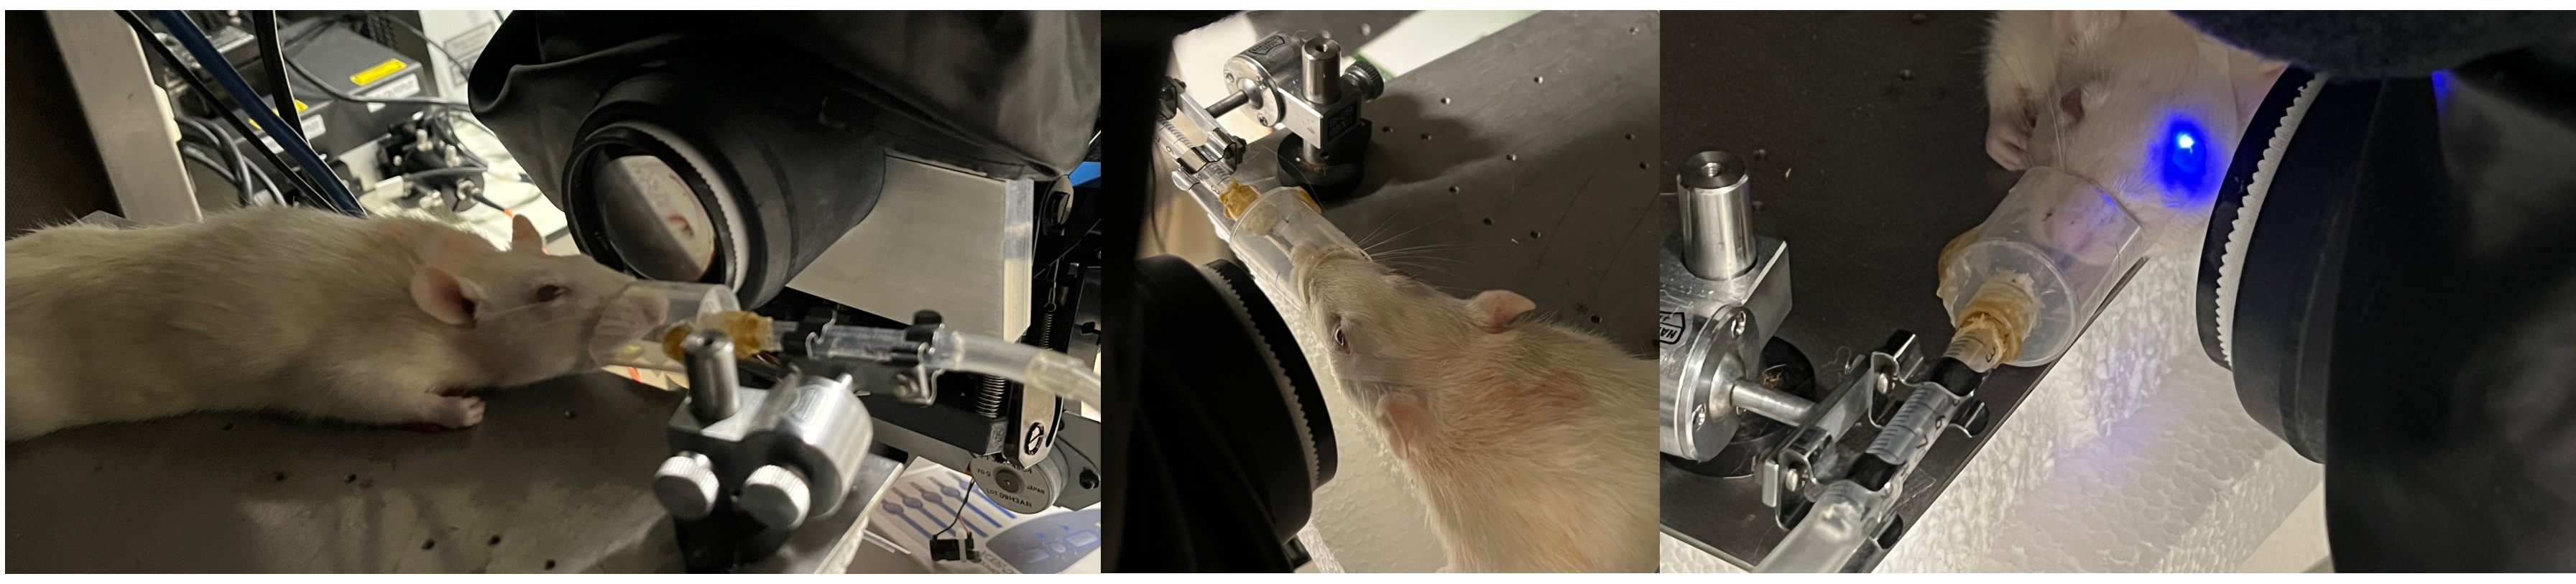
\includegraphics[width = \textwidth]{figures/ratUCL/RatSetupFigure.pdf}}
        \annotatedFigureText{0.015,0.83}{white}{0.3}{a)}
        \annotatedFigureText{0.435,0.83}{white}{0.3}{b)}
        \annotatedFigureText{0.66,0.83}{white}{0.3}{c)}
    \end{annotatedFigure}
    
    \caption{a) and b) The anaesthetised rat is positioned on the imaging platform perpendicular to the SFLIO system to have the rat's retina parallel with the image plane. The fundus camera is moved axially such that the illumination forms a focussed spot on the cornea - evenly illuminating the retina (c).}
    \label{fig:ratsetup}
\end{figure}
Three rats were imaged and for each rat, brightfield images are recorded continuously (\SI{50}{\ms} exposure at \SI{10}{\Hz}) in tandem with the FLIMera operating in raw mode over a two minute acquisition period for all 4 spectral filters. This SFLIM acquisition is carried out while the rats are cycled from a Normoxia to Hypoxia (\SI{15}{\percent}\ce{FiO2}) and then back to Normoxia again. SFLIM images were recorded for a single rat post-mortem. When changing oxygenation state each rat was allowed to stabilise for a period of 5 minutes to ensure that the concentration of retinal FAD was not changing during the image acquisition period.
As before (\cref{fig:flimerascmossync}), the two detectors are synchronised in time by initially having the laser shutter closed and then opening it after a short period of time and detecting the Heaviside-like change in photon flux. Due to the anaesthetic the nervous responses in the rats is suspended resulting in image sequences free of saccades and drifts. This lack of movement meant that in the motion compensation stage no pixel super-sampling was performed (\cref{fig:FLIMerareg}c).


\begin{figure}
    \centering
    \begin{annotatedFigure}{\includegraphics[width = \textwidth]{figures/ratUCL/RatsCMOSfigure.pdf}}
        \annotatedFigureText{0.025,0.91}{white}{0.3}{a)}
        \annotatedFigureText{0.35,0.91}{white}{0.3}{b)}
        \annotatedFigureText{0.68,0.91}{white}{0.3}{c)}
        \annotatedFigureText{0.19,0.425}{white}{0.3}{d)}
        \annotatedFigureText{0.52,0.425}{white}{0.3}{e)}
    \end{annotatedFigure}
    \caption{a - c) Shows exemplar brightfield images recorded of each of the 3 rats imaged. Each frame is recorded over an integration time of \SI{30}{\ms} at a rate of \SI{10}{\Hz} where a small amount of glare is present in the highlighted region of a). In d) and e) a fluorescence intensity image was recorded using a \SI{500}{\nm} longpass filter over integration times of \SI{1}{\second} and \SI{5}{\second} respectively.}
    \label{fig:Ratscmosimages}
\end{figure}


\subsection{Acquisition of SFLIM Images}

\section{}